%%% D\'ebut du pr\'eambule %%%

%%%%%%%%%%%%%%%%%%%%%%%%%%%%%%%%%
% Options g\'en\'erales du document %
%%%%%%%%%%%%%%%%%%%%%%%%%%%%%%%%%

\documentclass[12pt]{report}	% Classe du document

%%%%%%%%%%%%%%%%%%%%%%%
% Encodage, fontes... %
%%%%%%%%%%%%%%%%%%%%%%%

%\usepackage[latin1]{inputenc}
%\usepackage[utf8]{inputenc} 
\usepackage{amssymb}
\usepackage{bm}
\usepackage{latexsym}
\usepackage{amsmath}
%\usepackage{graphicx}
%\usepackage{aeguill}
%\usepackage{aecompl}
\usepackage{url}
\usepackage{scribe_MG}
 		% Encodage d'entr\'ee : permet l'utilisation de caract\`eres accentu\'es en entr\'ee




\usepackage{graphicx}			% pour les images
\usepackage{hyperref}
\hypersetup{
    bookmarks=true,         
    unicode=true,  
    colorlinks=true,       
    linkcolor=blue,          
    citecolor=blue,       
    filecolor=blue,      
    urlcolor=blue          
}

%%% Fin du pr\'eambule %%%


%%% Define new commands
\newcommand{\Ber}{\mathrm{Ber}}
\DeclareMathOperator*{\argmin}{\arg\!\min}
\DeclareMathOperator*{\argmax}{\arg\!\max}
\def\RR{\mathbb{R}}
\def\PP{\mathbb{P}}
\def\xb{\mathbf{x}}
\def\EE{\mathbb{E}}


% For the table of contents
%\makeatletter
%\newcommand*{\toccontents}{\vspace{1in}{\centering{\bf \large Contents}\bigskip \hrule \bigskip
%\noindent\@starttoc{toc} \bigskip \hrule }}
%\makeatother
%%% D\'ebut du document %%%

\begin{document}
\nocite{*}
	 
\scribe{Huu Dien Khue Le, Robin B\'enesse}		% required
\lecturenumber{1}			% required, must be a number
\lecturedate{October 9, 2013}		% required, omit year

	
\maketitle

The web page of the course: \url{http://www.di.ens.fr/~fbach/courses/fall2013/}

%\tableofcontents
%\toccontents
%\newpage

\section{Introduction}

\subsection{Problem}
To model complex data, one is confronted with two main questions:
\begin{itemize}
\item How to manage the complexity of the data to be processed?
\item How to infer global properties from local models?
\end{itemize}
These questions lead to 3 types of problems: the representation of data (or how to obtain a global model from a local model), the inference of the distributions (how to use the model), and the learning of the models (what are the parameters of the models?).

\subsection{Examples}
\BIT
\item \textbf{Image:} consider a $100 \times 100$ (pixels) monochromatic image. If each pixel is modelled by a discrete random variable (so there are 10000 of them), then the image can be modelled using a grid of the form:
\begin{figure}[ht]
\begin{center}
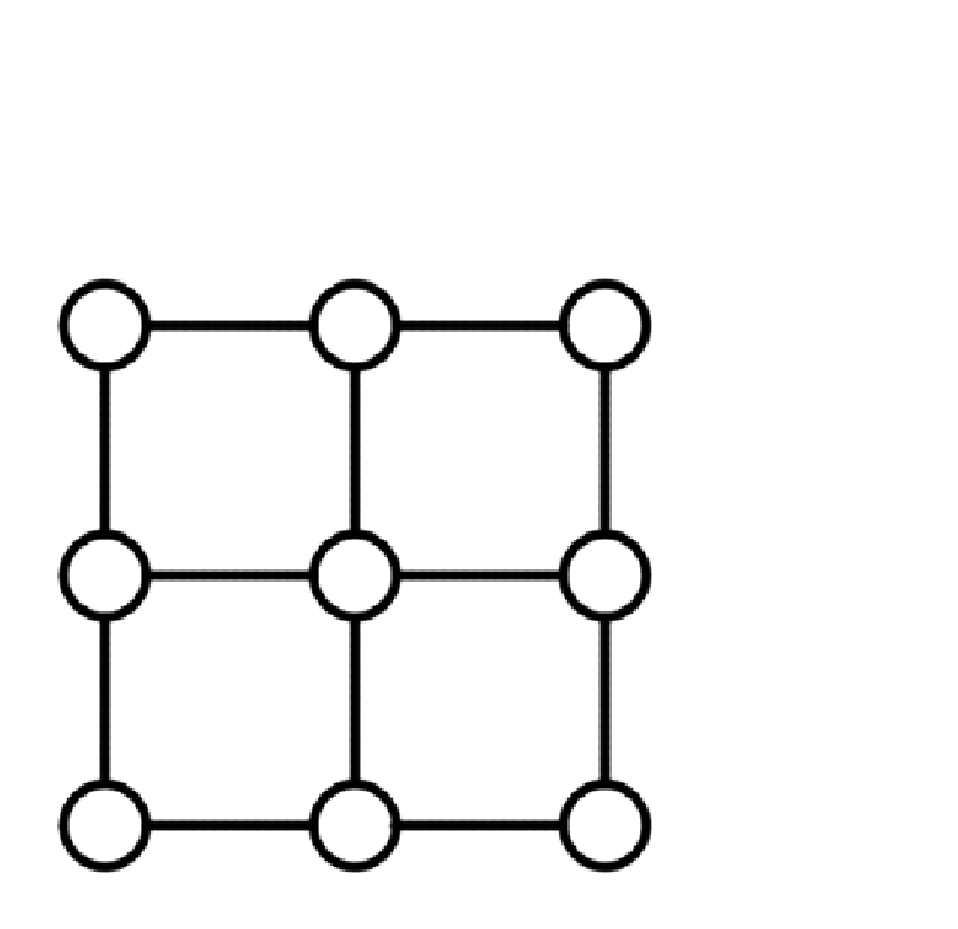
\includegraphics[angle=0, height=4cm]{graphe_image.pdf}
\end{center}
\centering
\end{figure}

\item \textbf{Bioinformatics:} consider a long sequence of $10000$ ADN bases. If each base of this sequence is modelled by a discrete random variable (that, in general, can take values in $\{A, C, G, T\}$), then the sequence can be modelled by a Markov chain:
\begin{figure}[ht]
\begin{center}
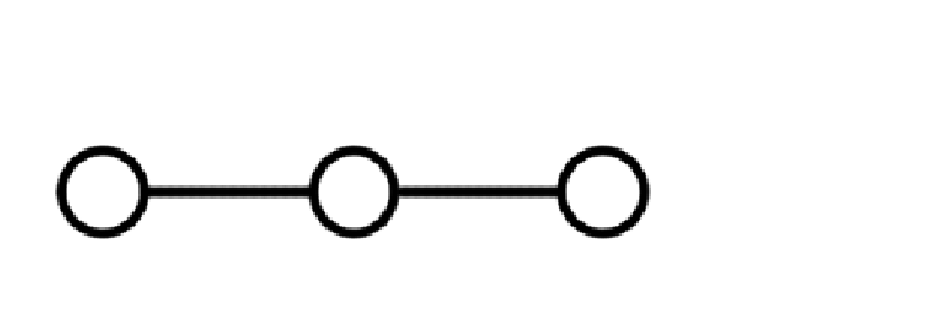
\includegraphics[angle=0, height=1.5 cm]{graphe_ADN.pdf}
\end{center}
\centering
\end{figure}

\item \textbf{Finance:} consider the evolution of stock prices in discrete time, where we have values at time $n$. It is reasonable to postulate that the change of price of a stock at time $n$ only depends only on its price (or the price of other stocks) at time $n-1$. For only two stocks, a possible simplified model is the following dependency graph:
\begin{figure}[ht]
\begin{center}
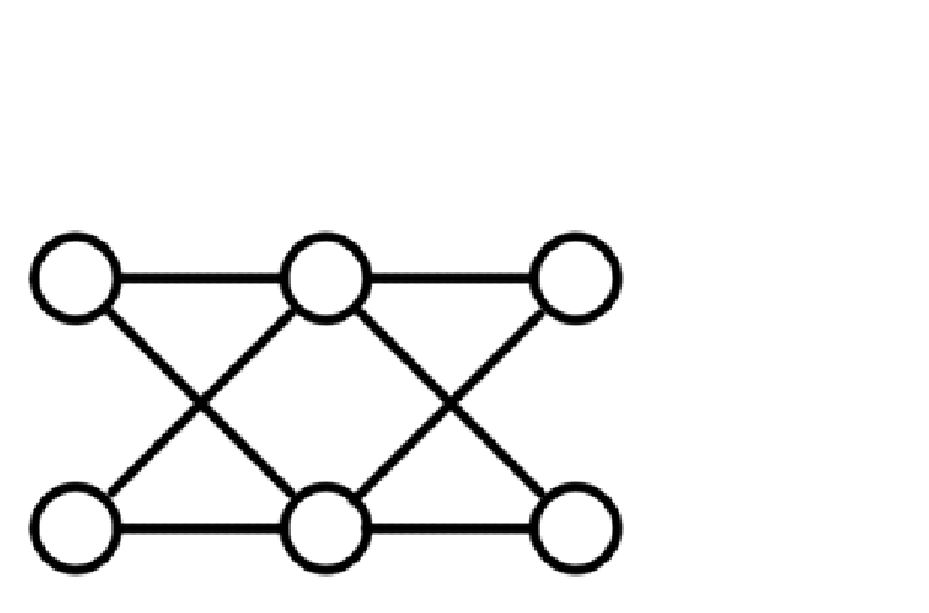
\includegraphics[angle=0, height=2.5 cm]{graphe_action.pdf}
\end{center}
\centering
\end{figure}

\item \textbf{Speech processing:} consider the syllables of a word and the way they are interpreted by a human ear or by a computer. Each syllable can be represented by a random sound. The objective is then to retrieve the word from the sequence of sounds heard or recorded. In this case, we can use a hidden Markov model:
\begin{figure}[ht]
\begin{center}
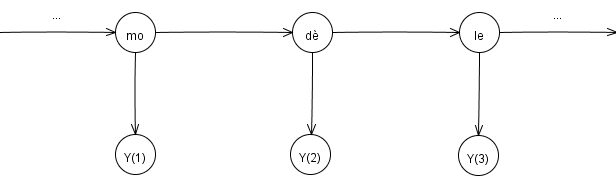
\includegraphics[angle=0, height=3cm]{graphe_parole.png}
\end{center}
\end{figure}


\item \textbf{Text:} consider a text with $1000000$ words. The text is modelled by a vector such that each of its components equals to the number of times each keyword appears. This is usually called the ``bag of words'' model. This model seems to be weak, as it does not take the order of the words into account. However, it works quite well in practice. A so-called \emph{naive Bayes classifier} can be used for classification (for example spam \emph{vs} non spam).\\
\end{itemize}

It is clear that models which ignore the dependence among variables are too simple for real-world problems. On the other hand, models in which every random variable is dependent all or too many other ones are doomed both for statistical (lack of data) and computational reasons. Therefore, in practice, one has to make suitable assumptions to design models with the right level of complexity, so that the models obtained are able to \emph{generalize} well from a statistical point of view and lead to tractable computations from an algorithmic perspective.

\section{Basic notations and properties}
In this section we recall some basic notations and properties of random variables.\\

\noindent {\textbf{Convention:}}  Mathematically, the probability that a random variable $X$ takes the value $x$ is denoted $p(X=x)$. In this document, we simply write $p(X)$ to denote a distribution over the random variable $X$, or $p(x)$ to denote the distribution evaluated for the particular value $x$. It is similar for more variables.


\begin{description}
\item[Fundamental rules.] For two random variables $X,Y$ we have
\begin{itemize}
\item Sum rule: $$p(X)=\sum_{Y}p(X,Y).$$
\item Product rule: $$p(X,Y)=p(Y|X)p(X).$$
\end{itemize}
\item[Independence.] Two random variables $X$ and $Y$ are said to be independent if and only if $$P (X,Y) = P(X) P(Y).$$
\item[Conditional independence.] Let $X,Y,Z$ be random variables. We define $X$ and $Y$ to be conditionally independent given $Z$ if and only if $$P (X,Y | Z)=P(X|Z)P(Y|Z).$$
\textit{Property:} If $X$ and $Y$ are conditionally independent given $Z$, then $$P(X|Y,Z)=P (X|Z).$$
\item[Independent and identically distributed.] A set of random variables is independent and identically distributed (i.i.d.) if each random variable has the same probability distribution as the others and all are mutually independent.
\item[Bayes formula.] For two random variables $X, Y$ we have $$P(X|Y)= \frac{P(Y|X)P(X)}{P(Y)}.$$
(Note that Bayes formula is not a Bayesian formula in the sense of Bayesian statistics).
\end{description}

\section{Statistical models}
\begin{definition}[Statistical model]
A (parametric) statistical model $\mathcal{P}_{\Theta}$ is a collection of probability distributions (or a collection of probability density functions\footnote{In which case, they are all defined with respect to the same base measure, such as the Lebesgue measure in $\RR^d$}) defined on the same space and parameterized by parameters $\theta$ belonging to a set $\Theta \subset \RR^p$. Formally:
$$\mathcal{P}_{\Theta}=\{p_\theta(\cdot) \mid \theta \in \Theta\}.$$
\end{definition}

\subsection{Bernoulli model}
Consider a binary random variable $X$ that can take the value 0 or 1. If $p(X=1)$ is parametrized by $\theta \in [0,1]$:
\begin{displaymath}
\left\{
    \begin{array}{ll}
        \PP(X=1)=\theta\\
        \PP(X=0)=1-\theta
    \end{array}
\right.
\end{displaymath}
then a probability distribution of the Bernoulli model can be written as

\begin{equation}
\label{eq:bernoulli}
p(X=x;\theta) = \theta^x(1-\theta)^{1-x}
\end{equation}
and we can write
\begin{equation}
X \sim \Ber(\theta).
\end{equation}

The Bernoulli model is the collection of these distributions for $\theta \in \Theta=[0,1]$.
\subsection{Binomial model}
A binomial random variable $\text{Bin}(\theta, N)$ is defined as the value of the sum of $n$ i.i.d.\ Bernoulli r.v. with parameter $\theta$. The distribution of a binomial random variable $N$ is 
$$\PP(N=k)=\binom{n}{k} {\theta}^k (1-\theta)^{n-k}.$$
The set $\Theta$ is the same as for the Bernoulli model.
\subsection{Multinomial model}
\label{subsec:multinomial}
Consider a discrete random variable $C$ that can take one of $K$ possible values $\{1,2,\ldots,K\}$. The random variable $C$ can be represented by a $K$-dimensional random variable $X=(X_1,X_2,\ldots,X_K)^T$ for which the event $\{C=k\}$ corresponds to the event $$\{X_k=1 \text{ and } X_l=0, \forall l \neq k\}.$$ \\
If we parametrize $\PP(C=k)$ by a parameter $\pi_k \in [0,1]$, then by definition we also have 
\begin{equation*}
\PP(X_k=1) = \pi_k \ \ \forall k=1,2,\ldots,K,
\end{equation*}
with $\sum_{k=1}^K \pi_k=1$. The probability distribution over $\xb=(x_1,\ldots, x_k)$ can be written as
\begin{equation}
\label{eq:multinomial}
p(\mathbf{x};\bm{\pi})=\prod_{k=1}^K\pi_k^{x_k}
\end{equation}
where $\bm{\pi}=(\pi_1,\pi_2,\ldots,\pi_K)^T$.  We will denote $\mathcal{M}(1,\pi_1, \ldots, \pi_K)$ such a discrete distribution. The corresponding set of parameters is $\Theta=\{\bm{\pi} \in \RR^+ \mid \sum_{k=1}^K \pi =1\}.$

Now if we consider $n$ independent observations of a $\mathcal{M}(1,\bm{\pi})$ multinomial random variable $X$, and we denote by $N_k$ the number of observations for which $x_k=1$, then the joint distribution of $N_1,N_2,\ldots,N_K$ is called a multinomial $\mathcal{M}(n,\bm{\pi})$ distribution. It takes the form:
\begin{equation}
p(n_1,n_2,\ldots,n_K;\bm{\pi},n)=\frac{n!}{n_1!n_2!\ldots n_K!} \prod_{k=1}^K\pi_k^{n_k}
\end{equation}
and we can write
\begin{equation}
(N_1,\ldots,N_K) \sim \mathcal{M}(N,\pi_1,\pi_2,\ldots,\pi_K).
\end{equation}

The multinomial $\mathcal{M}(n,\bm{\pi})$ is to the $\mathcal{M}(1,\bm{\pi})$ distribution, as the binomial distribution is to the Bernoulli distribution. In the rest of this course, when we will talk about multinomial distributions, we will always refer to a $\mathcal{M}(1,\bm{\pi})$ distribution.

\subsection{Gaussian models}
The Gaussian distribution is also known as the normal distribution. In the case of a scalar variable $X$, the Gaussian distribution can be written in the form
\begin{equation}
\label{eq:gaussian1}
\mathcal{N}(x; \, \mu,\sigma^2)=\frac{1}{(2\pi\sigma^2)^{1/2}}\exp\left(-\frac{(x-\mu)^2}{2\sigma^2}\right)
\end{equation} 
where $\mu$ is the mean and $\sigma^2$ is the variance. For a $d$-dimensional vector $\mathbf{x}$, the multivariate Gaussian distribution takes the form
\begin{equation}
\label{eq:gaussian2}
\mathcal{N}(\mathbf{x}|\bm{\mu},\bm{\Sigma})=\frac{1}{(2\pi)^{d/2}}\frac{1}{|\bm{\Sigma}|^{1/2}}\exp\left(-\frac{1}{2}(\mathbf{x}-\bm{\mu})^T\bm{\Sigma}^{-1}(\mathbf{x}-\bm{\mu})\right)
\end{equation}
where $\bm{\mu}$ is a $d$-dimensional vector, $\bm{\Sigma}$ is a $d\times d$ symmetric positive definite matrix , and $|\bm{\Sigma}|$ denotes the determinant of $\bm{\Sigma}$.
It is a well-known property that the parameter $\bm{\mu}$ is equal to the expectation of $X$ and that the matrix $\bm{\Sigma}$ is the covariance matrix of $X$, which means that $\bm{\Sigma}_{ij}=\EE[(X_i-\mu_i)(X_j-\mu_j)]$.


\section{Parameter estimation by maximum likelihood}
\subsection{Definition}
Maximum likelihood estimation (MLE) is a method of estimating the parameters of a statistical model. Suppose we have a sample $x_1,x_2,\ldots,x_n$ of $n$ independent and identically distributed observations, coming from a distribution $p(x_1,x_2,\ldots,x_n;\theta)$ where $\theta$ is an unknown parameter (both $x_i$ and $\theta$ can be vectors). As the name suggests, the MLE finds the parameter $\hat{\theta}$ under which the data $x_1,x_2,\ldots,x_n$ are most likely:
\begin{equation}
\hat{\theta} = \argmax_\theta p(x_1,x_2,\ldots,x_n; \, \theta) 
\end{equation}
The probability on the right-hand side in the above equation can be seen as a function of $\theta$ and can be denoted by $\mathcal{L}(\theta)$:
\begin{equation}
\mathcal{L}(\theta) = p(x_1,x_2,\ldots,x_n; \, \theta) 
\end{equation}
This function is called the \textit{likelihood}.\\
As $x_1,x_2,\ldots,x_n$ are independent and identically distributed, we have
\begin{equation}
\mathcal{L}(\theta) = \prod_{i=1}^n p(x_i; \, \theta) 
\end{equation}
In practice it is often more convenient to work with the logarithm of the likelihood function, called the \textit{log-likelihood}:
\begin{align}
\ell(\theta) = \log\mathcal{L}(\theta) 	&= \log \prod_{i=1}^n p(x_i; \, \theta) \\ 
						&= \sum_{i=1}^n \log p(x_i; \, \theta) \label{eq:loglikelihood}
\end{align}

Next, we will apply this method for the models presented previously. \textbf{We assume that all the observations are independent and identically distributed} in all of the remainder of this lecture.

\subsection{MLE for the Bernoulli model}
Consider $n$ observations $x_1,x_2,\ldots,x_n$ of a binary random variable $X$ following a Bernoulli distribution $\Ber(\theta)$. From \eqref{eq:loglikelihood} and \eqref{eq:bernoulli} we have 
\begin{align*}
\ell(\theta) 	&= \sum_{i=1}^n \log p(x_i; \, \theta) \\
				&= \sum_{i=1}^n \log \theta^{x_i}(1-\theta)^{1-x_i}\\
				&= N\log(\theta)+(n-N)\log(1-\theta)
\end{align*} 
where $N=\sum_{i=1}^n x_i$.\\ 
As $\ell(\theta)$ is strictly concave, it has a unique maximizer, and since the function is in addition differentiable, its maximizer $\hat\theta$ is the zero of its gradient $\nabla \ell(\theta)$: 
$$\nabla \ell(\theta)=\frac{\partial}{\partial\theta} \ell(\theta) = \frac{N}{\theta}-\frac{n-N}{1-\theta}.$$  
It is easy to show that $\nabla \ell(\theta) = 0 \Longleftrightarrow \theta =\frac{N}{n}$. Therefore we have 
\begin{equation}
\hat{\theta} = \frac{N}{n} = \frac{x_1+x_2+\cdots+x_n}{n}.
\end{equation} 

\subsection{MLE for the multinomial model}
Consider $N$ observations $X_1,X_2,\ldots,X_N$ of a discrete random variable $X$ following a multinomial distribution $\mathcal{M}(1,\bm{\pi})$, where $\bm{\pi} = (\pi_1,\pi_2,\ldots,\pi_K)^T$. We denote $\mathbf{x}_i$ ($i=1,2,\ldots,N$) the $K$-dimensional vectors of 0s and 1s representing $X_i$, as presented in Section~\ref{subsec:multinomial}. \\
From  \eqref{eq:loglikelihood} and \eqref{eq:multinomial} we have
\begin{align*}
\ell(\bm{\pi}) 	&= \sum_{i=1}^N \log p(\mathbf{x}_i; \, \bm{\pi}) \\
				&= \sum_{i=1}^N \log \left( \prod_{k=1}^K\pi_k^{x_{ik}} \right)\\
				&= \sum_{i=1}^N \sum_{k=1}^K x_{ik} \log  \pi_k\\
				&= \sum_{k=1}^K n_k \log  \pi_k
\end{align*}
where $n_k=\sum_{i=1}^N x_{ik}$ ($n_k$ is therefore the number of observations of $x_k=1$).\\
We need to maximize this quantity subject to the constraint $\sum_{k=1}^K \pi_k = 1$.\\

\subsubsection*{Brief review on Lagrange duality}
\begin{description}
\item[Lagrangian.] Consider the following convex optimization problem:  
\begin{equation}
\label{eq:convex-prob}
\min_{\mathbf{x}\in \mathcal{X}} f(\mathbf{x}), \text{ subject to }	\mathbf{Ax=b}
\end{equation}
where $f$ is a convex function, $\mathcal{X} \subset \mathbb{R}^p$ is a convex set included in the domain\footnote{The domain of a function is the set on which the function is finite.} of $f$,  $\mathbf{A}\in \mathbb{R}^{n\times p}, \mathbf{b}\in \mathbb{R}^{n}$.\\
The \textit{Lagrangian} associated with this optimization problem is defined as
\begin{equation}
\label{eq:lagrangian}
L(\mathbf{x},\bm{\lambda})= f(\mathbf{x}) + \bm{\lambda}^T(\mathbf{Ax-b})
\end{equation}
The vector $\bm{\lambda} \in \mathbb{R}^n$ is called the \textit{Lagrange multiplier vector}.\\

\item[Lagrange dual function.] The \textit{Lagrange dual function} is defined as 
\begin{equation}
\label{eq:dual-function}
g(\bm{\lambda}) = \min_{\mathbf{x}} L(\mathbf{x},\bm{\lambda})
\end{equation}
The problem of maximizing $g(\bm{\lambda})$ with respect to $\bm{\lambda}$ is known as the \textit{Lagrange dual problem}.\\ 

\item[Max-min inequality.]For any $f:\mathbb{R}^n\times \mathbb{R}^m$ and any $w\in \mathbb{R}^n$ and $z\in \mathbb{R}^m$, we have
\begin{align}
f(w,z) \le \max_{z\in Z} f(w,z) &\Longrightarrow \min_{w\in W} f(w,z) \le \min_{w\in W} \max_{z\in Z} f(w,z) \\
&\Longrightarrow \max_{z\in Z}\min_{w\in W} f(w,z) \le \min_{w\in W} \max_{z\in Z} f(w,z). \label{eq:max-min-ineq} 
\end{align}
The last inequality is known as the \textit{max-min inequality}.\\ 

\item[Duality.] It is easy to show that
\begin{align*}
\max_{\bm{\lambda}}L(\mathbf{x},\bm{\lambda}) = 
\begin{cases} f(\mathbf{x}) &\mbox{if } \mathbf{Ax=b} \\ 
			 +\infty				& \mbox{otherwise.} 
\end{cases}
\end{align*}
Which gives us
\begin{equation}
\label{eq:minmax}
\min_{\mathbf{x}} f(\mathbf{x}) = \min_{\mathbf{x}} \max_{\bm{\lambda}}L(\mathbf{x},\bm{\lambda})
\end{equation}
Now from \eqref{eq:dual-function}, \eqref{eq:max-min-ineq} and \eqref{eq:minmax} we have
\begin{equation}
\label{eq:weak-dual}
\max_{\bm{\lambda}} g(\bm{\lambda}) = \max_{\bm{\lambda}} \min_{\mathbf{x}} L(\mathbf{x},\bm{\lambda}) \le \min_{\mathbf{x}} \max_{\bm{\lambda}} L(\mathbf{x},\bm{\lambda}) = \min_{\mathbf{x}} f(\mathbf{x})
\end{equation}  
This inequality says that the optimal value $d^*$ of the Lagrange dual problem always lower-bounds the optimal value $p^*$ of the original problem. This property is called the  \textit{weak duality}. If the equality $d^*=p^*$ holds, then we say that the  \textit{strong duality} holds. Strong duality means that the order of the minimization over $\mathbf{x}$ and the maximization over $\bm{\lambda}$ can be switched without affecting the result.

\item[Slater's constraint qualification lemma.] If there exists an  $\mathbf{x}$ in the relative interior of $\mathcal{X} \cap \{\mathbf{Ax=b}\}$ then strong duality holds. (Note that by definition $\mathcal{X}$ is included in the domain of $f$ so that if $\xb \in \mathbf{X}$ then $f(\xb)<\infty$.)
\end{description}

Note that all the above notions and results are stated for the problem \eqref{eq:convex-prob} only. For a more general problem and more details about Lagrange duality, please refer to \cite{Boyd04} (chapter 5). 

\subsubsection*{Back to our problem}
We need to minimize
\begin{equation}
f(\bm{\pi}) = -\ell(\bm{\pi}) = -\sum_{k=1}^K n_k \log  \pi_k
\end{equation}
subject to the constraint $\mathbf{1}^T\bm{\pi}=1$.\\
The Lagrangian of this problem is
\begin{equation}
L(\bm{\pi},\lambda)= -\sum_{k=1}^K n_k \log  \pi_k + \lambda\left(\sum_{k=1}^K\pi_k -1\right)
\end{equation}

Clearly, as $n_k \ge 0$ ($k=1,2,\ldots,K$), $f$ is convex and this problem is a convex optimization problem. Moreover, it is trivial that there exist $\pi_1,\pi_2,\ldots,\pi_K$ such that $\pi_k > 0$ ($k=1,2,\ldots,K$) and $\sum_{k=1}^K\pi_k=1$, so by \emph{Slater's constraint qualification}, the problem has strong duality property. Therefore, we have
\begin{equation}
\min_{\bm{\pi}} f(\bm{\pi}) = \max_\lambda\min_{\bm{\pi}} L(\bm{\pi},\lambda)
\end{equation}
As $L(\bm{\pi},\lambda)$ is convex with respect to $\bm{\pi}$, to find $\min_{\bm{\pi}} L(\bm{\pi},\lambda)$, it suffices to take derivatives with respect to $\pi_k$. This yields $$\frac{\partial L}{\partial\pi_k} = -\frac{n_k}{\pi_k}+\lambda =0, \ k=1,2,\ldots,K.$$
or
\begin{equation}
\label{eq:pik}
\pi_k = \frac{n_k}{\lambda},\ k=1,2,\ldots,K.
\end{equation}
Substituting these into the constraint $\sum_{k=1}^K \pi_k = 1$ we get $\sum_{k=1}^K n_k = \lambda$, yielding $\lambda = N$. From this and \eqref{eq:pik} we get finally
\begin{equation}
\hat\pi_k = \frac{n_k}{N},\ k=1,2,\ldots,K.
\end{equation}
\textit{Remark:} $\hat\pi_k$ is the fraction of the $N$ observations for which $x_k=1$.

\subsection{MLE for the univariate Gaussian model}
Consider $n$ observations $x_1,x_2,\ldots,x_n$ of a random variable $X$ following a Gaussian distribution $\mathcal{N}(\mu,\sigma^2)$. From \eqref{eq:loglikelihood} and \eqref{eq:gaussian1} we have 
\begin{align*}
\ell(\mu,\sigma^2) 	&= \sum_{i=1}^n \log p(x_i; \, \mu,\sigma^2) \\
				&= \sum_{i=1}^n \log\left[ \frac{1}{(2\pi\sigma^2)^{1/2}}\exp\left(-\frac{(x_i-\mu)^2}{2\sigma^2}\right)\right]\\
				&= -\frac{n}{2}\log(2\pi)-\frac{n}{2}\log(\sigma^2)-\frac{1}{2}\sum_{i=1}^n \frac{(x_i-\mu)^2}{\sigma^2}.				
\end{align*} 
We need to maximize this quantity with respect to $\mu$ and $\sigma^2$. By taking derivative with respect to $\mu$ and then $\sigma^2$, it is easy to obtain that the pair $(\hat{\mu},\hat{\sigma}^2)$, defined by
\begin{align}
\hat{\mu}&=\frac{1}{n}\sum_{i=1}^n x_i \\
\hat{\sigma}^2&=\frac{1}{n}\sum_{i=1}^n \left(x_i-\hat{\mu}\right)^2
\end{align}
is the only stationary point of the likelihood. One can actually check (for example computing the Hessian w.r.t.~$(\mu,\sigma^2)$ that this actually a maximum. We will have a confirmation of this in the lecture on exponential families.  

\subsection{MLE for the multivariate Gaussian model}
Let $X \in \mathbb{R}^d$ be a Gaussian random vector, with mean vector $\mu\in\mathbb{R}^{d}$ and a covariance matrix $\Sigma\in\mathbb{R}^{d\times d}$ (positive definite):
\BEAS
p(x\;|\;\mu,\Sigma) = \frac{1}{\left(2\pi\right)^{\frac{k}{2}}} \frac{1}{\sqrt{\det\Sigma}} \exp\left(\frac{-\left(x- \mu \right)^\top \Sigma^{-1} \left( x - \mu \right)}{2}\right)
\EEAS
Let $x_1, \dots, x_n$ be a i.i.d. sample. The log-likelihood is given by:
\BEAS
\ell\left( \mu, \Sigma \right) & = & \log p\left(x_1, \dots, x_n; \, \mu,\Sigma\right) \\ 
& = & \log \prod_{i=1}^n p \left(x_i \;|\; \mu, \Sigma \right)\\ 
& = & - \left(\frac{nd}{2}\log(2\pi) + \frac{n}{2}\log\left(\det \Sigma \right) + \frac{1}{2}\sum_{i=1}^n\left(x_i-\mu\right)^\top\Sigma^{-1}\left(x_i-\mu\right)\right)
\EEAS
In this case, one should be careful that these log-likelihoods are not concave with respect to the pair of parameters $(\mu, \Sigma)$. They are concave w.r.t.~$\mu$ when $\Sigma$ is fixed but they are not even concave with respect to $\Sigma$ when $\mu$ is fixed.
\subsection{Digression: review on differentials}

\noindent\textbf{Differentiable function.} A function f is differentiable at $x\in\mathbb{R}^{d}$ if there exists a linear form $df$ such that: 
$$ f(x+h) - f(x) = df(h) + o(||h||)$$

~\\
Since $\mathbb{R}^{d}$ is a Hilbert space, we know that there exists $g\in\mathbb{R}^{d}$ such that $df_{x}(h) = \langle g,h\rangle$. We call $g$ the gradient of $f$ : $g = \nabla f(x)$.\\
~\\
Example 1 : if $f\mapsto a^{\top} x + b$ then we have : 

$$ f(x+h) - f(x) = a^\top h $$ and thus $$ \nabla f(x) = a.$$
~\\
Example 2 : if $f\mapsto \frac{1}{2}x^{\top} Ax$ then we have : 

\BEAS
f(x+h) - f(x) & = & \frac{1}{2}(x+h)^{T}A(x+h)-\frac{1}{2}x^{\top}Ax \\ 
& = &  \frac{1}{2}\left(x^{\top}Ah + h^{\top}Ax\right) + o\left(||h||\right)  \\ 
\EEAS
The gradient is then : 

$$\nabla f(x) = \frac{1}{2}\left(Ax + A^{\top}x \right)$$

Let us first differentiate $\ell\left( \mu, \Sigma \right)$ w.r.t. $\mu$.\\

We need to differentiate : 

$$\mu\mapsto (x_{i}-\mu)^{\top}\Sigma^{-1}(x_{i}-\mu)$$
~\\
Which is equal to $f \circ g$ where :\\

\begin{center}
$\begin{array}{ccccc}
f & : & \mathbb{R}^{d} & \to & \mathbb{R} \\
  &   & y & \mapsto & y^{\top}\Sigma^{-1}y \\
\end{array}$
\end{center}
and 

\begin{center}
$\begin{array}{ccccc}
g & : & \mathbb{R}^{d} & \to & \mathbb{R}^{d} \\
  &   & \mu & \mapsto & \mu - x_{i} \\
\end{array}$
\end{center}
~\\
\underline{Reminder : Composition of differentials}

\BEAS
d(f\circ g) & = & df_{g(x)}\left(dg_{x}(h)\right) \\ 
						& = & df_{g(x)}\circ dg_{x}(h) 								 
\EEAS

The differential of f is : $df_{y}(h) = \langle\nabla f(y),h\rangle = \langle\frac{1}{2}\left(\Sigma^{-1}y+\left(\Sigma^{-1}\right)^{\top}y\right),h\rangle = \langle\Sigma^{-1}y,h\rangle$

as $\Sigma^{-1}$ is symmetric.\\
~\\
The function $\ell : \mu\mapsto (x_{i}-\mu)\Sigma^{-1}(x_{i}-\mu)$. We have : 

$$d\ell_{\mu}(h) = \langle \Sigma^{-1}(\mu - x_{i}), h \rangle$$

We deduce the gradient of $\ell$ : 

$$\nabla\ell(\mu) = \Sigma^{-1}(\mu - x_{i})$$

\subsection{Back to the MLE for the multivariate Gaussian }

Remember that the function we want to differentiate is : 

$$\ell\left( \mu, \Sigma \right) = - \left(\frac{nd}{2}\log(2\pi) + \frac{n}{2}\log\left(\det \Sigma \right) + \frac{1}{2}\sum_{i=1}^n\left(x_i-\mu\right)^\top\Sigma^{-1}\left(x_i-\mu\right)\right)$$

According to the results above, we have :

\BEAS
\nabla_{\mu}\ell\left(\mu,\Sigma^{-1}\right) & = & \sum_{i=1}^{n} \Sigma^{-1}(\mu - x_{i}) \\ 
& = & \Sigma^{-1}\left(n\mu - \sum_{i=1}^{n} x_{i}\right)\\ 
& = & \Sigma^{-1}\left(n\mu - n\overline{x}\right)
\EEAS

where $\overline{x} = \frac{1}{n}\sum_{i=1}^{n}x_{i}$\\
~\\
The gradient is equal to 0 iff : 

$$\boxed{\widehat{\mu} = \frac{1}{n}\sum_{i=1}^{n}x_{i}}$$
~\\
Let us now differentiate $\ell$ w.r.t. $\Sigma^{-1}$. Let $A = \Sigma^{-1}$. We have : 

$$\ell\left( \mu, \Sigma \right) = - \left(\frac{nd}{2}\log(2\pi) - \frac{n}{2}\log\left(\det A \right) + \frac{1}{2}\sum_{i=1}^n\left(x_i-\mu\right)^\top A\left(x_i-\mu\right)\right)$$

The last term is a real number, so it equal to its trace. Thus : 

\BEAS
\ell\left( \mu, \Sigma \right) & = & - 
\left(\frac{nd}{2}\log(2\pi) - \frac{n}{2}\log\left(\det A \right) + \frac{1}{2}\sum_{i=1}^{n} \textrm{Trace}\left((x_i-\mu)^\top A(x_i-\mu)\right)\right) \\
& = & - \left(\frac{nd}{2}\log(2\pi) - \frac{n}{2}\log(\det A) + \frac{n}{2}\textrm{Trace}(A\widetilde{\Sigma})\right)
\EEAS

where $$\widetilde{\Sigma} = \frac{1}{n}\sum_{i=1}^{n}(x_{i}-\mu)(x_{i}-\mu)^{\top}$$

is the empirical covariance matrix.\\

Let $f : A\mapsto \frac{n}{2}\textrm{Trace}\left(A\widetilde{\Sigma}\right)$.\\
~\\
We have : 

$$f(A+H) - f(A) = \frac{n}{2}\textrm{Trace}\left(H\widetilde{\Sigma}\right)$$

The gradient of the last term of $\ell$ is then :

$$\nabla f(A) = \frac{n}{2}\widetilde{\Sigma}$$

and : 

\BEAS 
df_{A}(H) & = & \langle\nabla f(A),H\rangle\\
& = & \textrm{Trace}\left(\nabla f(A)^{\top}H\right)
\EEAS

Let us focus on the second term. We have : 

\BEAS \log\left(\det(A+H)\right) & = & \log\left(|A^{\frac{1}{2}}\left(I + A^{-\frac{1}{2}}HA^{-\frac{1}{2}}\right)A^{-\frac{1}{2}}|\right) \\
& = & \log\left(|A|\right) + \log\left(\det(I+\widetilde{H})\right)
\EEAS

where $\widetilde{H} = \left( A^{-\frac{1}{2}}\right)HA^{-\frac{1}{2}}$.\\
~\\
Let $g : A\mapsto \log\left(\det(A)\right)$ where $A = I + \widetilde{H}$.\\

We have : 

\BEAS
\log\left(\det(I+\widetilde{H})\right) - \log\left(\det(I)\right) & = & \sum_{i=1}^{d}\log(1+\lambda_{j}) \\
& \simeq & \sum_{i=1}^{d} \lambda_{j} + o\left(||\widetilde{H}||\right) \\
& = & \textrm{Trace}\left(\widetilde{H}\right) + o\left(||\widetilde{H}||\right)
\EEAS

$\widetilde{H}$ is symmetric, so it can be written as : 

\BEAS
\widetilde{H} = U\Lambda U^{\top}
\EEAS
 
where U is an orthogonal matrix and $\Lambda = \textrm{diag}(\lambda_{1},...,\lambda_{d})$.\

$$\textrm{d}\left(\log\left(\textrm{det}_{A}(H)\right)\right) = \textrm{Trace}\left(A^{-\frac{1}{2}}HA^{-\frac{1}{2}}\right) = \textrm{Trace}(HA^{-1})$$

We deduce the gradient of $\log\left(\det(A)\right)$:

$$\nabla\log\left(\det(A)\right) = A^{-1}$$

And the gradient of $\ell$ w.r.t. A is : 

$$\nabla_{A}(\ell) = -\frac{n}{2}A^{-1} + \frac{n}{2}\widetilde{\Sigma}$$

It is equal to zero iff : 

$$\widehat{\Sigma} = \widetilde{\Sigma}$$

when $\widetilde{\Sigma}$ is invertible. 

Finally we have shown that the pair
$$\hat{\mu}=\bar{x}=\frac{1}{n} \sum_{i=1}^n x_i \quad \text{and} \hat{\Sigma}=\frac{1}{n} \sum_{i=1}^n (x_i-\bar{x})(x_i-\bar{x})^\top$$
is the only stationary point of the likelihood. One can actually check (for example computing the Hessian w.r.t.~$(\mu,\Sigma)$ that this actually a maximum. We will have a confirmation of this in the lecture on exponential families.  
\bibliographystyle{unsrt}
\bibliography{biblio}
\end{document}
%%% Fin du document %%%
	
